\documentclass[12pt]{article}
\usepackage{graphicx}
\usepackage{enumerate}% http://ctan.org/pkg/enumerate
\usepackage[top = 1.25 in, bottom = 1.25 in, left=1.3 in, right = 1.3in]{geometry}
\usepackage{setspace}
\usepackage{float}
\usepackage{algpseudocode}
\usepackage{cleveref}

\usepackage{amsmath}

\begin{document}

\title{An Agent Based Model for Competitive Equilibrium in Electricity Markets\\ \small{Submitted for Undergraduate Thesis in Economics\\ Spring 2015}}


\author{Michael Lee \\{\small Advised by: Dr. Valerie Bencivenga\thanks{ Senior Lecturer, Department of Economics, The University of Texas at Austin}}}


\maketitle{}
\thispagestyle{empty}
\newpage{}
\pagenumbering{roman}


\begin{center}Abstract\end{center}

The research presented herein aims to computationally model participants in an electric utilities market. Utilizing an agent based (AB) approach, players are treated as uniquely intelligent, independent agents who seek to maximize utility via selective bidding in a marketplace. Agents must decide thier optimal output based on expectations of their opponent's quantities supplied, the carbon make up of said supply, as well as expectations of future carbon tax rates. In making their decisions, agents are able to look back at historical quantity supplied, as well as look into their own cost structures in order to predict future outcomes. Agents are also able to invest and divest selectively from assets, giving them additional agency in affecting their outcomes. \*

Fundamental basis of the model come from various economic models, including oligopolistic competition-- specifically Carnout competition-- and Walrasian auctioning. The former denotes the market structure where firms decide independently on the output they will supply, while the later describes the mechanism by which competitors find equilibrium via repeated bidding. \*


The model is accomplished via a mix of computational tools, specifically python and its associated libraries. The prediction mechanism is achieved through multiple regression, while all optimization is performed via linear algebra toolkits. In order to increase efficiency in calculations, the model can be performed in parallel across many cores, assigning each agent and its associated properties to a single core for computation. 

Results show that the speed in which agents reach a steady state is inversely proportional to the number of market participants, the decrease in consumer price per megawatt as the number of market participants increases, the the rate at which marginal taxes on carbon effect production on participants of different scales. These results are inline with the expectations put forth by optimization theory, Cornout competition, and Pigovian taxes. \*
 
\newpage

\begin{center}Acknowledgments \end{center}
A special shout to Dr. Bencivenga for her help through this progressively stressful experience, as well as her valuable insight into the best way to get from JFK to ERW during the holidays.
\newpage
\tableofcontents
 
\newpage 

\listoffigures

\newpage

\doublespacing
\pagenumbering{arabic}
% =========================================================== % 
\section{Competitive Equilibrium in Electricity Markets}
The change from government-regulated to competitive electric markets  created a market structure that shares more similarities with a oligopoly than a truly competitive market. In 1989, the United Kingdom passed the Electricity Act of 1989 which provided for the privatization of the electricity industry in Great Britain. Sixteen years later, California passes the Electric Utility Industry Reconstruction Act with the purported goal of increasing competition with dire effects. Since then, much work has been dedicated to understanding and modeling electric markets. \*


\begin{figure}[H]
	\begin{center}
	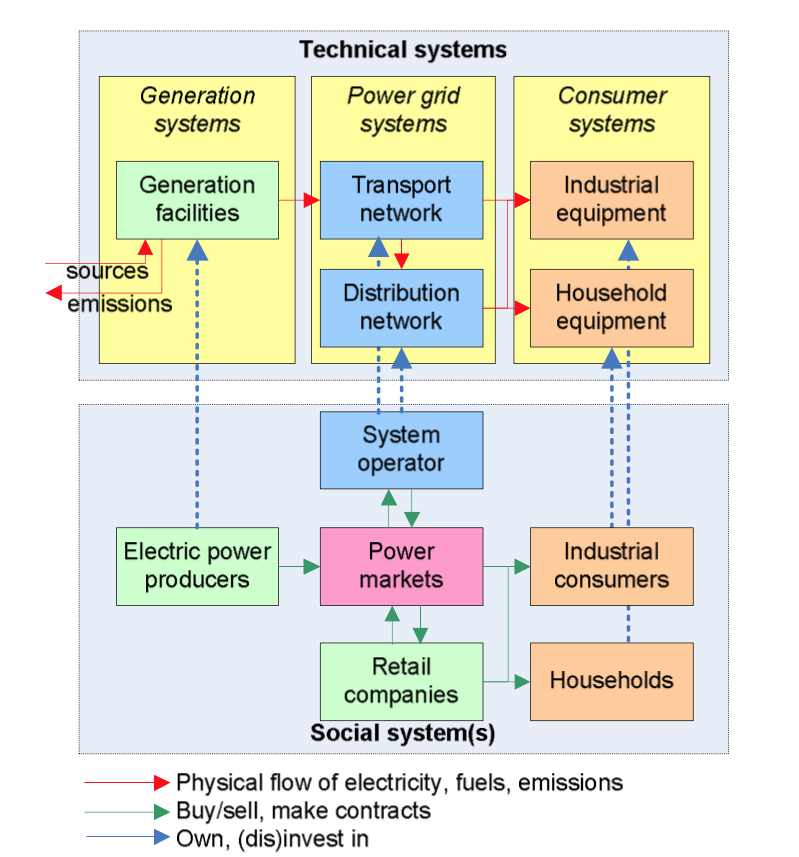
\includegraphics[scale = .3]{cetMarket}
	\caption{Electric Markets and Their Constituent Systems \cite{flowfig}}
	\label{cetMarket}
	\end{center}
\end{figure}

\Cref{cetMarket} shows the relationship between various systems within the electric market. The flow of electricity, and therefor emissions, travels from the industrial producers of electricity-- who primarily rely on fossil fuels for their heat source-- through the distribution networks to the homes and offices of the consumer. The generation facilities are the focus of this research, specifically their design making as to scale and fuel source in a competitive environment. 

\subsection{Market Equilibrium}
Competitive equilibrium in the model is defined as the state in which there are no changes in production levels between iterations. At each iteration, all sellers in the market decide on a level of production that will produce the highest utility given a known demand curve and an \emph{expected} aggregate electricity supply. At the end of each iteration, all bids are summed, the price is calculated, and agents decide if they over or underproduced based on their individual production costs. Computationally, the algorithm that settles production acts as a market manager, more specifically a Walrasian auctioneer.\*

Each agent is treated as uniquely intelligent, using the output of previous rounds to adjust their expectations until a steady-state competitive equilibrium is reached. This process is a mirror of a Walrasian auction: instead of each agent calculating demand at all possible prices, all agents simultaneously submit bids for how much they are willing to produce at each possible price point. If after all bids have been submitted, and an agent's market expectations are above the actualized quantities, it will subsequently lower its productions proportional to the difference between the two amounts. In the computational model, this process is performed via a negative feedback loop.\footnote{See \cref{feedback}}\*


\subsubsection{The Asymmetric Information Problem}\label{asymmetry}
One of the critical problems with modeling electric markets is the dependence on all parties of perfect information regarding their rivals cost structures. Since electricity markets are primarily a margins-driven business, producers can only operate when the cost per-megawatt is above their production costs. However, since production is sent to an "electric pool", where multiple producer's output is amalgamated, the optimal production bundle of each agent is dependent on the summation of all bids in the market, and therefore the  marginal costs of all producers. If agents cannot perfectly know all other participant's cost structure, they will not be able to accurately predict the aggregate supply, and suboptimal production will result. 


\subsection{Market Structure: Competitive or Oligopolistic}
It has been argued that the competitive equilibrium model is only applicable in markets in which there are a large number of sellers. In small markets-- like they one modeled here-- each player's production dramatically influences the market price. This market power to alter the price means that the market functions similar to an oligopoly.\*

The market modeled has properties similar to a Cournot oligopoly, namely: output is homogenous and chosen simultaneously across all firms, firms act independently, firms are price setters, and firms seek to maximize utility given opponent's actions. Critically, the underlying assumption of the Cournot model is the "not" conjecture, i.e. that the firm takes the output of its competitors as given and that its own production decision will not effect its competitor's production outcomes.\footnote{\Cref{feedback} shows how this assumption is implemented in the computational model.} \*

\subsection{Potential Models}

Previous work into oligopolistic electricity markets have utilized the Cournot, Bertrand, Stackelberg, supply function equilibrium (SFE) and collusion models. Similar to the model presented herein, Hogan and Cardel \emph{et al} use a Cournot quantity approach to a single period of market trading \cite{hogan}. Building off this approach, Chen, Wong \emph{et al} created a coevolutionary computational (CCEM) model in which two players evolve in the power "ecosystem" based on their fitness, which in this case is a profit function\cite{chen}. \*

Agent-based computational economics (ACE) is a particularly well-suited platform for capturing the dynamic interaction between many different agents. In ACE, each market participant is modeled as an agent who is given a utility function that it seeks to maximize at each interval. One downside of this model however, is that that it its most basic form, the players cannot form any strategic 'thinking' based on previous turns. ACE can be combined with other forms of computational modeling, specifically genetic algorithms (GA) to produce "smart" models. \*

\subsubsection{Argonne National Laboratory EMCAS}
Researchers at Argonne National Laboratory (ANL) Decision and Information Sciences developed a software tool that models participants in an electric market. The Electricity Market Complex Adaptive System (EMACAS) models "heterogeneous, decentralized decision structures"\cite{EMCAS} as agents, each with their own set of objectives and decision making rules. The expanded model can use both historical data (e.g. previous prices) as well as predict future prices. EMCAS is a complete software suite, complete with a GUI and programmable agent characteristics. ECMAS is a commercially available and has been used by 1300+ users working across the gamut of enterprises, including the Illinois Commerce Commission. \*

\begin{figure}[H]
	\begin{center}
	\includegraphics[scale = .75]{EMCAS}
	\caption{EMCAS Flow Diagram \cite{EMCAS}}
	\end{center}
\end{figure}

The work contained herein follows a similar approach to that of EMCAS, utilizing an agent-based approach to the power markets. The overlap between the two projects can be used to validate the techniques and approach used in the model presented in this paper.

  
% =========================================================== % 

\section{Carbon Dioxide Production}


One of the goals of this model is to show how a marginal carbon tax can effect the pollution outcomes of the market. In the model, agents predict total carbon emissions and use this information to plan their production. Since the tax rate is dependent on the total supply, agents are incentivized to work together and keep carbon output at or below the predefined tax threshold.\footnote{See \cref{carbon} for a detailed explanation of agent's $CO_2$ expectations} \*

\subsection{The Carbon Problem}
Over the past 100 years the global temperature has risen $1.53\,^{\circ}\mathrm{F}$. However, since ocean temperature tends to rise slower than land, the overall effect is more pronounced for Earth's landmasses. 

\begin{figure}[H]
	\begin{center}
	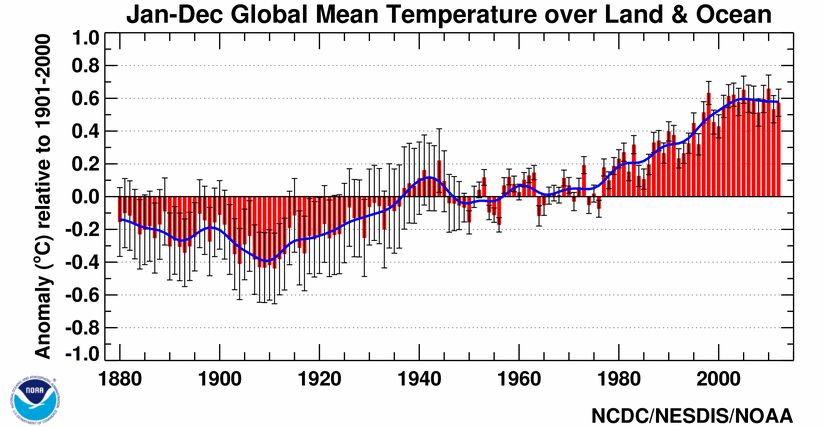
\includegraphics[scale = .4]{meantemp.png}
	\caption{Rise in Global Temperatures Since 1880 \cite{Temps}}
	\end{center}
\end{figure}

While there are those who contest the science, the vast majority of climatologists attribute this sustained rise in global temperatures to the increased use of fossil fuels for transportation and power. In the US, the largest source of these $CO_{2}$ emissions come from the generation of electric power followed by transportation. \footnote{The global average of $CO_{2}$ emissions from electric generation is roughly $\frac{1}{3}$)}

\begin{figure}[H]
	\begin{center}
	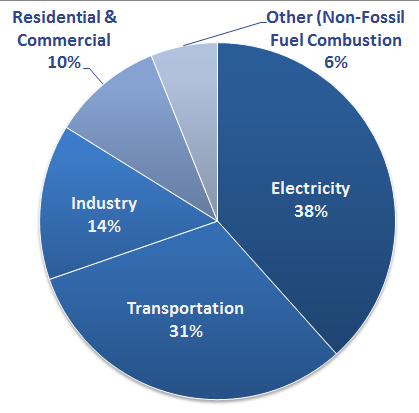
\includegraphics[scale = .4]{gases-co2.png}
	\caption{Breakdown of Greenhouse Gas Emissions by Source \cite{co2}}
	\end{center}
\end{figure}

\subsection{Efforts Towards a Carbon Tax}
A carbon tax is a mechanism which aims to disincentivize the production of greenhouse gases (GHGs) via raising the cost of pollution. GHGs represent a negative externality, and therefore taxation can be used to more accurately reflect the social cost of carbon-- a form of taxation known as a Pigovian tax after economist Arthur Pigou\cite{pigou}. \*

In the United States, there is no nationwide tax on carbon, however some municipalities have enacted a true carbon tax. In 2008, the Bay Area, California passed a 0.044 USD tax per tonne of carbon, however this fee is well below the suggested price of 40-60 USD per tonne\cite{co2tax}. 


\section{Model Formulation}
An agent based model is created in which multiple power providers independently select output based on expectations of future market conditions: including CO2 emissions, aggregate supply, and the regulatory environment. The market price per megawatt and effective tax rate are set via the value and composition of aggregate supply-- meaning each producer must at every turn accurately predict the combined output and its associated carbon emissions in order to choose its own optimal production bundle. If the combined carbon output is greater than an exogenous, known threshold, then a marginal tax on carbon is enacted. \* 

In the system, agents are aware of the market clearing price (MCP) and use thier own cost structure coupled with historical bids to estimate their opponet's future bidding behavior. In this sense, agents are able to "look back" and "look in" in order to formulate their optimal bids for the next period\footnote{Or, to "look forward"}. Agents seek to optimize their utility for time period $t+1$ by placing bids such that their utility-- a combination of revenue, utilization rate and emissions--is maximized in the market place. 

\subsection{Agent Characteristics}
Each member of the class \emph{agent} has the following unique attributes: 

	\begin{enumerate}
		\item Quantity of various production assets 
		\item Cost of production of each asset
		\item Utility Coefficients
		\item Available liquidity for investment
		\item Damping coefficient
	\end{enumerate} 

The characteristics listed above are variable for each agent and are initialized at the beginning of the simulation. All of the characteristics, except the utility coefficients, are dynamic and are updated as the simulation progresses. In the case where the above are identical for all agents, the quantities produced are the same for all agents and the steady state solution is immediately achieved \footnote{This is derived from the fact that producers use their own cost structure to as their initial guess of opponent's production.}.


\subsection{Optimal Production}
At each turn, agents find the optimal production via a simple utility function given their expectations of future output. Where \emph{U} is the total utility, \emph{R} is the revenue, \emph{C} is the carbon emissions, \emph{u} is the utilization rate, and $\alpha, \beta, \gamma $ are the utility coefficients for each:

	\begin{equation}
		\max_{\forall q \in Q} U_i(R, C, u) = \alpha_{i} R_{i} + \beta_{i} C_{i} + \gamma_{i} u_{i}
	\end{equation}

\subsubsection{Expected Revenue}
Expected revenue for each player, \emph{i}, is calculated as a function of the cost per megawatt-hour for each production technology \emph{j}, the quantity of each production technology supplied by player \emph{i}, and the expected market price, $P^{exp.}$, for electricity--  a function of aggregate supply, $S_{agg}$. In the model, a generic, linear demand curve is given, from which the market price is determined. 

	\begin{equation}
		P^{exp.}_{i} = 10 + .2S_{agg}^{exp.}
	\end{equation}

	\begin{equation}
		R^{exp.}_{i} = P^{exp.}_{i}Q_{i} - \sum_{j=0}^{N} c_{i}^{j}*q^{j}_{i} - \tau C_i
	\end{equation}

Where $Q_{i}$ is the total production for agent $i$, $c_i$ is the marginal cost of production for generation technology $j$, $\tau$ is the marginal tax rate\footnote{The relative costs of each table can be found in \cref{levelized}}, $C_{i}$ is the agent's carbon emissions, and $q$ is the quantity of each generation technology produced by the agent.\*

In the original and most simplified version of the model, the demand curve is exogenous, known, and static.

\subsubsection{Expected Carbon Emissions}\label{carbon}
Similar to expected revenue, agents also calculate the expected carbon emissions for each turn. Since agents face a marginal tax rate if and only if total carbon emissions are above a predefined threshold, the optimal production bundle will be influenced by expected carbon emissions. 

	\begin{algorithmic}
		\If {$C_{agg.} \geq C_{max}$}
			\State $tax = C^{CO2}_i * \tau$
		\Else
			\State $tax=0$
		\EndIf
	\end{algorithmic}
Of the three different production technologies, only natural gas produces CO2 \footnote {Natural gas produces 117 lbs of CO2 per million BTU \cite{co2}}. This implies that should an agent predict carbon emissions to be above the threshold, they will shift production towards clean technologies. Where $\kappa$ is the amount of CO2 produced per megawatt-hour by burning natural gas:

	\begin{equation}
		CO2^{exp.}_{i} = CO2^{exp.}_{opp} + q^{CO2}_{i}*\kappa
	\end{equation}

In the expanded game, agents also predict whether the tax rate and threshold will change in the future, as they must plan investment into different power generation facilities. As the expectations that the carbon tax will increase, agents move capital away from natural gas facilities and towards renewable energies. Where $\tau$ is the carbon tax rate, \emph{T} is the maximum amount of carbon allowable, $p_1$ is the probability that the tax rate increases, $p_2$  is the probability that the tax rate is less than or equal to its current level, $p_a$ is probability that the threshold decreases, and $p_b$ is the probability that the threshold is greater than or equal to its current levels:

	\begin{multline}\label{EV}
		E_{gas}[\tau, T] = P^{future}*Q_{gas} - [p_1\tau (Q_{gas} - p_aT) + p_2\tau (Q_{gas} - p_bT) \\+ p_1\tau (Q_{gas} - p_bT) + p_2\tau (Q_{gas} - p_aT)]
	\end{multline}

 Eq. 5 is the expected value operator for the agent's investment decision. Thus, the future regulatory environment and the accuracy of which agents can know it have dramatic effects on the outcome of the game.   


\subsubsection{Utilization Rate}
The final component of agent's utility is the utilization rate, defined as: 

	\begin{equation}
		u_{i} = \sum_{j=1}^{N}1 - \frac{A_{j}-q_{j}}{A_{j}}
	\end{equation}

Where $A_{j}$ is the total amount of asset $j$ that the agent owns.\*
The utilization rate is incorporated to ensure that agents are less inclined to disregard one asset type all together. In this sense, the utilization rate can be thought of as a minimum production diversification metric. Adding the utilization rate into the utility function also serves to keep agents from foregoing using their existing assets. 


\subsection{Cost Structure}
The costs of production vary with the type of generation technology used. However, in order to mimic the benefits of scale, the marginal cost for all types decreases with the total amount of assets the producer has. Ergo the more gas plants an agent has, the lower the marginal cost of producing electricity from natural gas. 

\subsection{Investment}
In the expanded model, agents may divest themselves from certain assets as well as "research" improved methods for generation. Based on the the existing portfolio of power generation and the benefits of shifting towards various types of production, agents may sell off assets at depreciated values or reinvest profits into lowering the cost per megawatt of a certain technology-- effectively investing in more capacity. \* 

The addition of future investment alters the utility calculations of agents. Since investment or divestment will effect optimal bundles for remainder of the game, agents must calculate the total utility gained or lost for the next five periods \footnote{In actuality, agents would need to calculate the utility for an infinite time horizon. However, for simplicity, agents predict that the game will last another five turns, regardless of the actual number of turns remaining}. Agents choose to invest or divest in technologies based on their current and previous utilization rates of technologies, as well as their expectations of the carbon tax rate and the amount of carbon produced in the future. To look forward, agents use a multiple regression algorithm to predict utility based on the expectations of the aforementioned variables. Thus at every turn, each agent calculates the utility gained over five periods for all permutations of buying, selling, or maintaining each asset. \\


	\begin{algorithmic}
		\For{\texttt{asset in Assets}}
			\State $\sum_{t=1}^{5}U_i^{sell}$

			\For{\texttt{asset in Remaining Assets}}
			\State $\sum_{t=1}^{5}U_i^{invest}$
				\For{\texttt{asset in Remaining Assets}}
					\State $\sum_{t=1}^{5}U_i^{maintain}$
		\EndFor
		\EndFor
		\EndFor
		\State \texttt{Find max permutation}
	\end{algorithmic}



\subsection{Modifying Expectations}
Players are unaware of their opponent's utility coefficients and their cost structure, thus they are unable to accurately predict at what quantity their opponents will produce at (\cref{asymmetry}). This imperfect information causes players to under or over produce which causes less than expected utility. In order to minimize this differential, after each turn players compare their expected aggregate supply to the actualized value. Players will dampen or amplify their production proportional to the delta they experience. 


	\begin{figure}[ht!]
		\begin{center}
		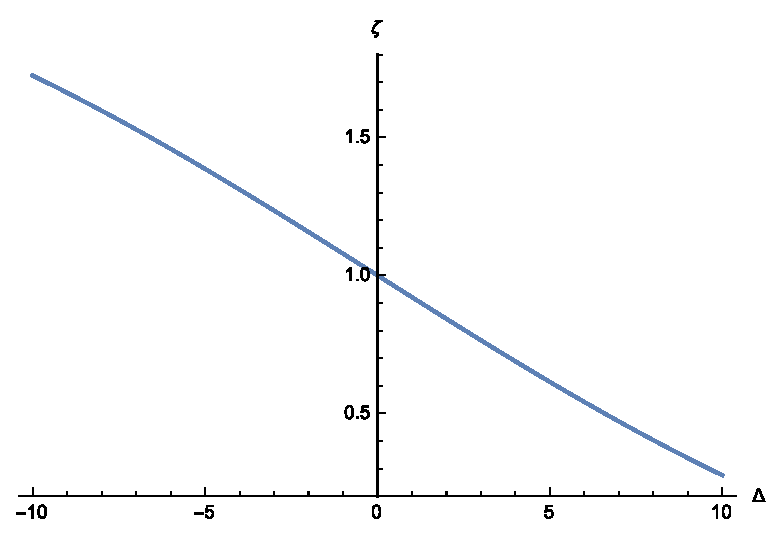
\includegraphics[scale = .6]{DF.eps}
		\caption{Expected Supply Damping Function}
		\end{center}
	\end{figure}

When delta is negative and the agent has overproduced, the agent will modify their future expectations by $\zeta > 1$. In the opposite situation, and the agent has underproduced, they will modify their future expectations by $\zeta < 1$. As the solution approaches steady state, $\delta$ will converge to zero and $\zeta$ converges to unity (\cref{results1}). 

	\begin{figure}[ht!]
		\begin{center}
		\includegraphics[scale = .6]{feedbackloop.png}
		\caption{Block Diagram of Feedback Loop}
		\label{feedback}
		\end{center}
	\end{figure}

 \Cref{feedback} details how the negative feedback loop is implemented. The optimization routine takes expected supply as an input and finds the optimal production bundle based on these expectations. After bid submission, the comparator finds the difference in expectation vs. reality and sends the result to the damping function. The damping function in-turn, creates a suitable damping ratio and multiplies it to the previous expectations to create future expectations. 

 	\begin{equation}
 		Q_{t+1}^{exp} = \zeta Q_{t}^{exp}
 	\end{equation}


% =========================================================== % 

\section{Achieved Results}
The first series of tests consisted of two agents, each with different utility coefficients, available assets, and cost structures. Agent \emph{1}, show in green, is the larger of the two producers\footnote{Agent \emph{2} is shown in blue}, and has the majority of its production capacity in natural gas. There are differences in the utility coefficients, however they are not extreme.\footnote{Recall that the closer the costs and coefficients are, the faster steady state will be reached}

	\begin{figure}[ht!]
		\begin{center}
		\includegraphics[scale = .75]{2Player.eps}
		\caption{Summary of Results, Case 1}
		\label{results1}
		\end{center}
	\end{figure}

\Cref{results1} shows the results of the baseline simulation. Here, you can see that $ \alpha $ quickly converges to unity as $\delta$ converges to nil. Agent \emph{1}, the larger of the two producers, becomes the dominate player in the market with approximately 70\% market share. In the model, fast convergence is indicative of  two agents being able to quickly 'feel out'\footnote{In Walras' words, 'tatonnement', or 'groping'} the opponent's optimal production bundle via the auction mechanism. Since there are only two agents, both players are able to identify their opponent's best production bundle with certainty by simply attributing all residual supply to the opponent. As the market expands, it can be shown that this methodology fails (\cref{competetion}). \*

	\begin{figure}[ht!]
		\begin{center}
		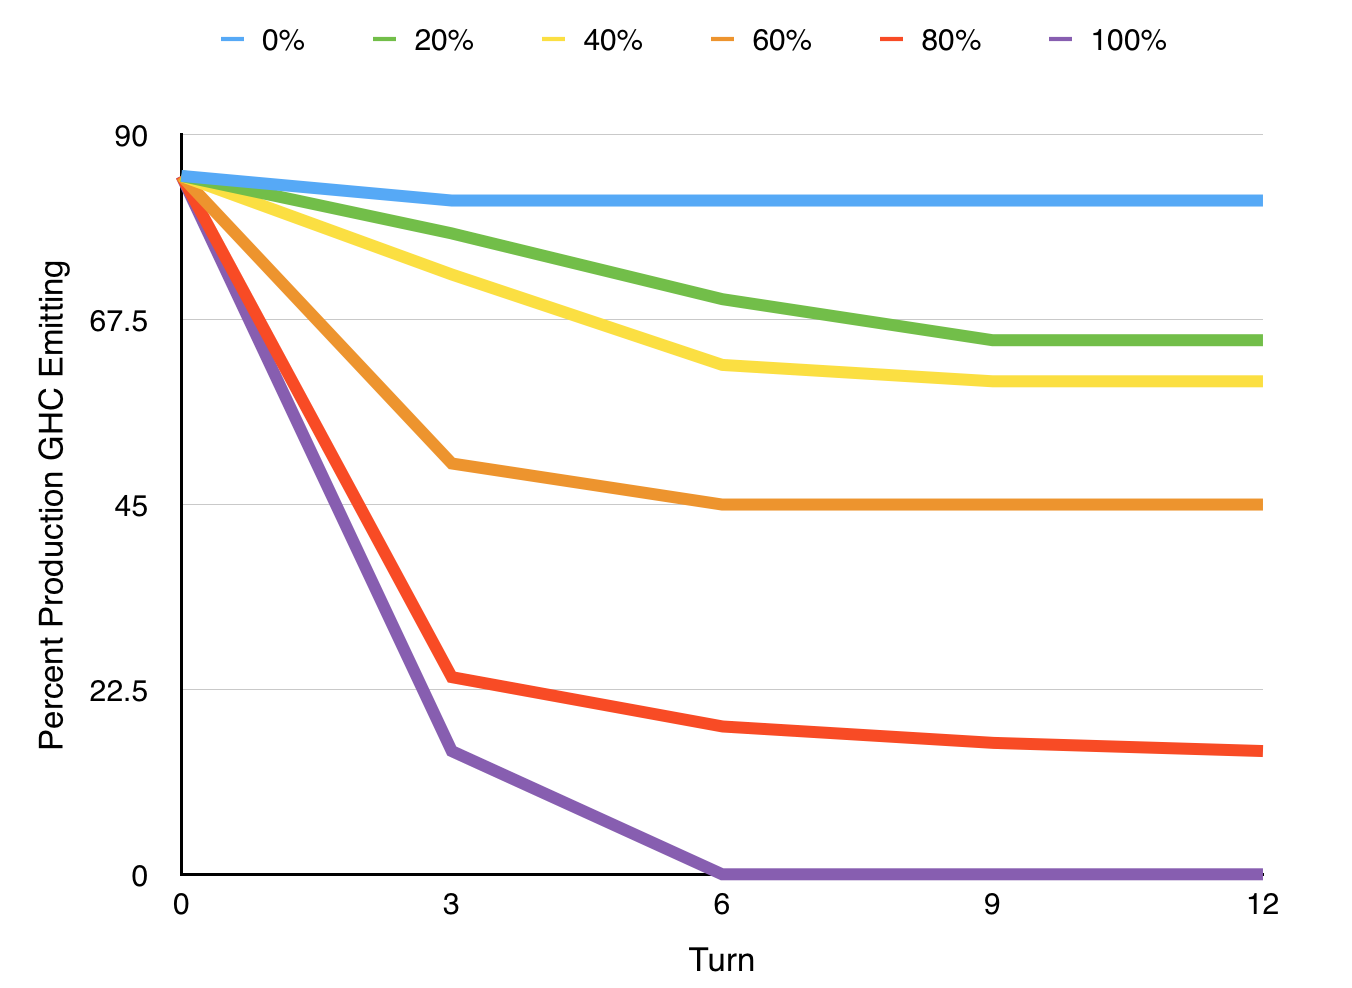
\includegraphics[scale = .4]{investment.png}
		\caption{Percent Polluting in Portfolios for Various Tax Rates, Case 1}
		\label{results2}
		\end{center}
	\end{figure}

\Cref{results2} shows the percentage of polluting technologies in the agent's portfolio as a function of the turn for various tax rates. As expected, when the tax rate is equal to the cost of natural gas, using gas becomes unprofitable and agents quickly divest from it. The sharp decline in emissions seen for an eighty percent tax rate suggest that the optimal tax rate is somewhere between 60\% and 80\% of the price of natural gas.

\subsection{Handling Market Expansion} \label{competetion}
The model is expandable and can handle an arbitrary number of players in the market \footnote{However, past four players the algorithm is no longer critically damped, and continues to oscillate around a fixed average; see \cref{5Players}}. However, as the number of agents increases, the amount of iterations required to reach a steady state increases too, as the damping function must now incorporate multiple variable outputs. Numerically, the model becomes more sensitive to initial conditions and less stable.\footnote{Here stability refers the ability for the algorithm to converge to its limit} and as a result, the model requires the all agent's initial conditions to be closer together. 


	\begin{figure}[ht!]
		\begin{center}
		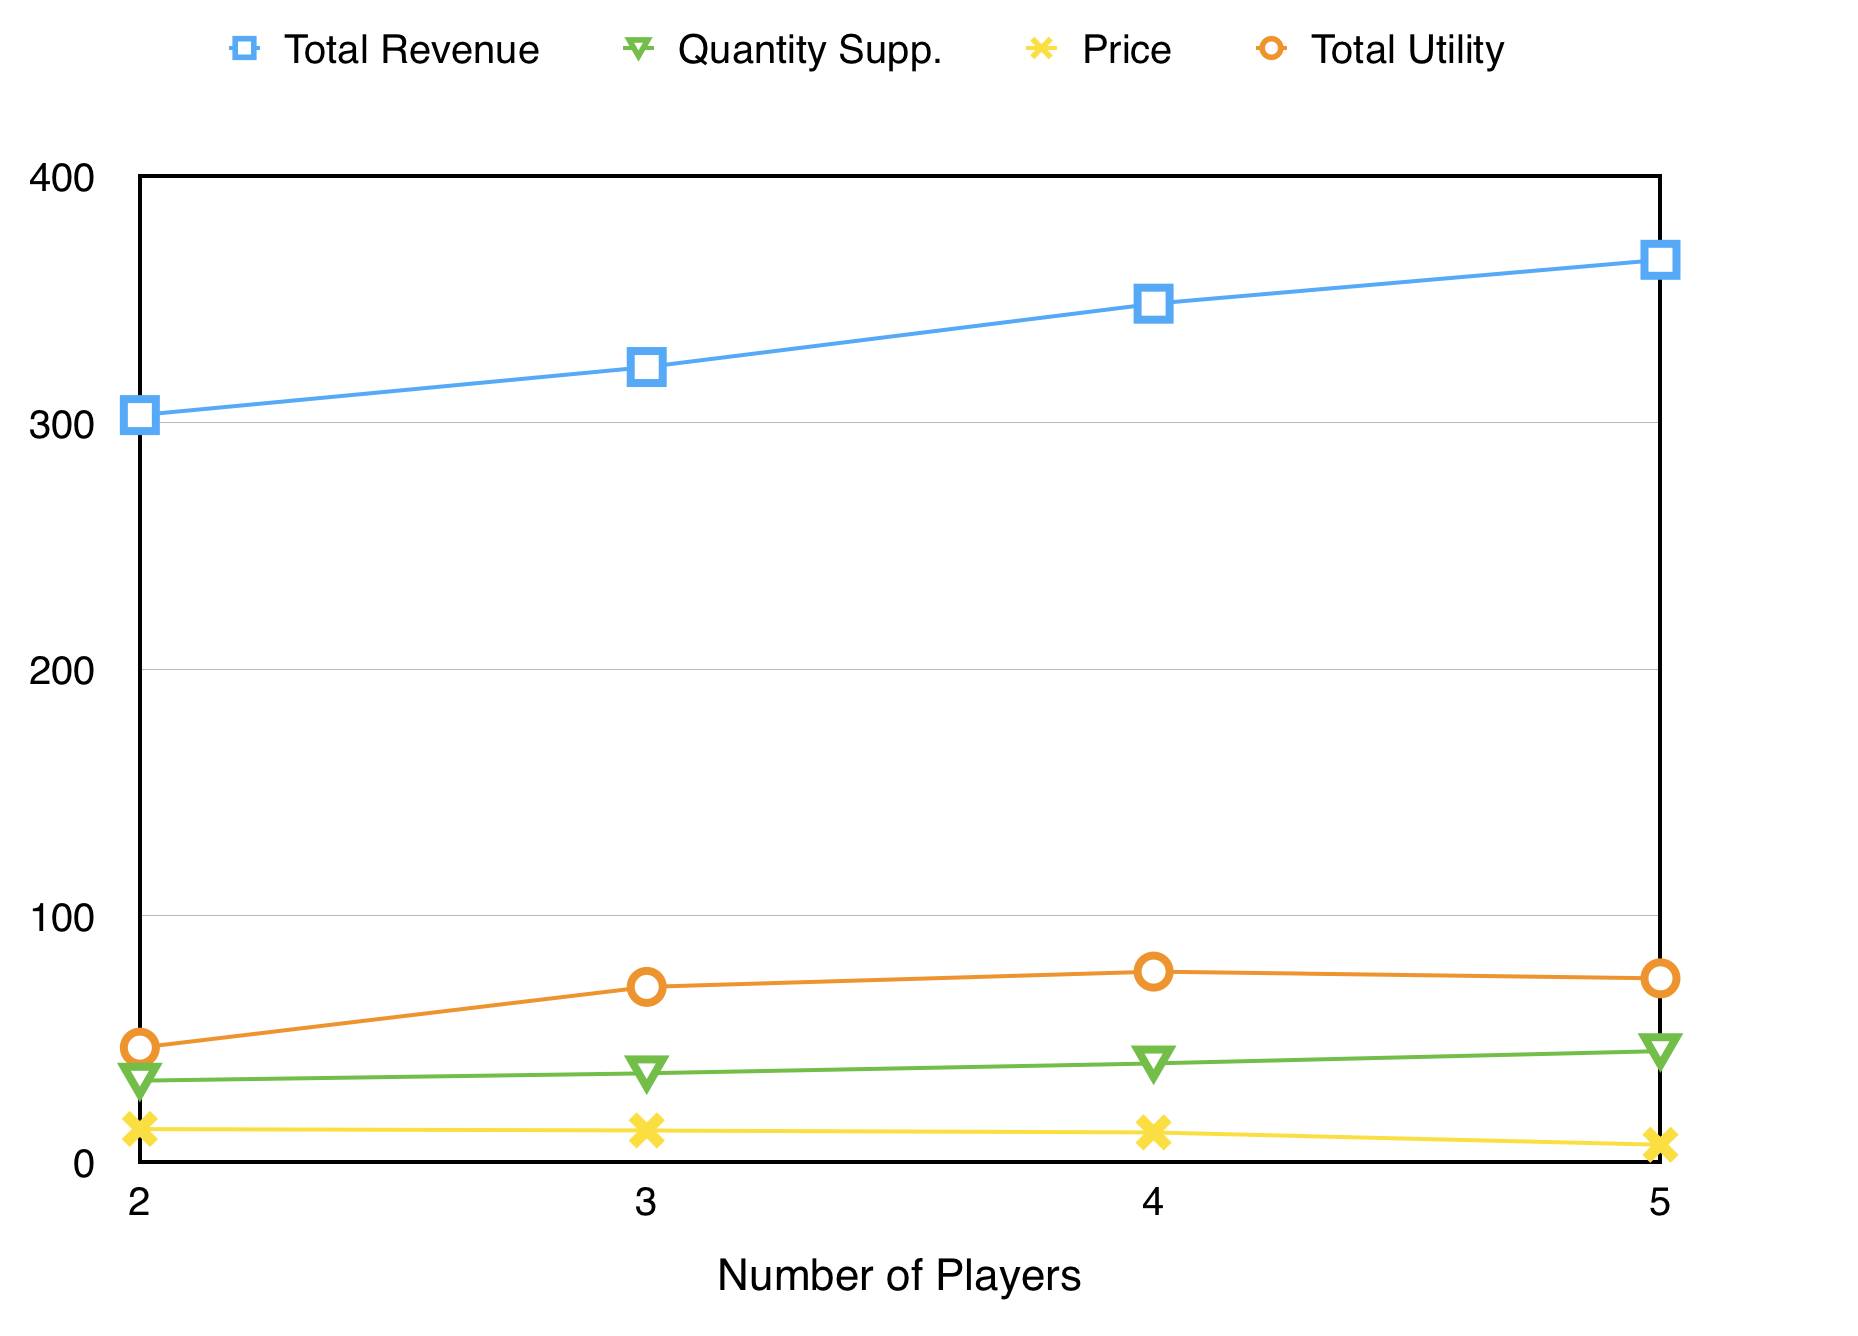
\includegraphics[scale = .45]{numP.png}
		\caption{Model Quantities as a Function of the Number of Players}
		\label{numP}
		\end{center}
	\end{figure}

\Cref{numP} shows how various quantities in the model react as the number of players increases. As expected, the price falls as N, the number of players, increases. This price decrease is accompanied by a subsequent increase in both the combined revenue of all agents and the total utility. This is inline with expectations of how oligopolies act: they  supply an artificially low quantity of goods such that they may maximize there own individual profit. As the number of players increases, competition brings the prices down until the competitive equilibrium price and quantity is reached. The Cournot theorem validates this outcome, stating that as the number of firms in the market goes to infinity, the quantity supplied goes to the competitive level and the price will converge to marginal cost.

	\begin{equation}
		\lim_{N\to\infty} Q^{oligopoly} = Q^{competitive}
	\end{equation}

While the total utility and revenue is higher as the number of players increases, no one agent has is able to significantly increase its own share of the gains. Thus, while the end consumer would win in the form of lower utility prices and higher power availability, the power producers will generate less revenue as the number of power providers increases. \*

Another unwanted side effect of decreased competition is an increase in the amount of carbon produced. As mentioned before, as the number of agents decreases, players are able to guess their opponent's moves with higher and higher certainty. At each iteration, agents chose their own carbon output based on what they expect their opponent's to produce (\cref{carbon}). The inverse relationship between players and certainty of outcomes forces agents to become more cautious with their carbon output with a larger number of players, since it is harder to account for how much carbon will be produced. It follows then that, for $N>2$ the total carbon output was zero, as firms were forced to be more cautious with $CO_2$ production. For $N \leq 2$, the amount of carbon production is always equal to the maximum allowable before the marginal tax is enacted.\* 

The reduction of carbon achieved by competition is counter-intuitive, especially since the overall size of the electricity market grows. However, the results indicate that the asymmetric information presented to producers will cause them to be overly cautious and produce emission free so long as the price differential between emitting and non-emitting technologies is small. It can also be argued that the increased number of players made it more difficult for the participants to collude in thier carbon production.

\subsection{Effects of Taxation on Producers of Different Scales} \label{scale}

The second experiment that the model was used for was to see how a carbon tax would effect producers of different sizes. Two agents were created, a smaller producer and a much larger one. In order to isolate the effects of scale, both producers had the same percentage of each generation type in their portfolio. The hypothesis was that large producers would be still be able to produce using polluting technologies as they would be able to leverage their scale into lower input prices. Smaller producers, would be forced into using non-emitting generation, and subsequently face smaller profit margins. This anticipated result would be counterproductive to the policy's spirit: large polluters could keep polluting at a higher rate since other market competitors would be priced out, and smaller, more environmentally-friendly players would be disincentivized since they would have smaller profit margins using more expensive technology and pooled pricing. \*

\begin{figure}[ht!]
	\begin{center}
	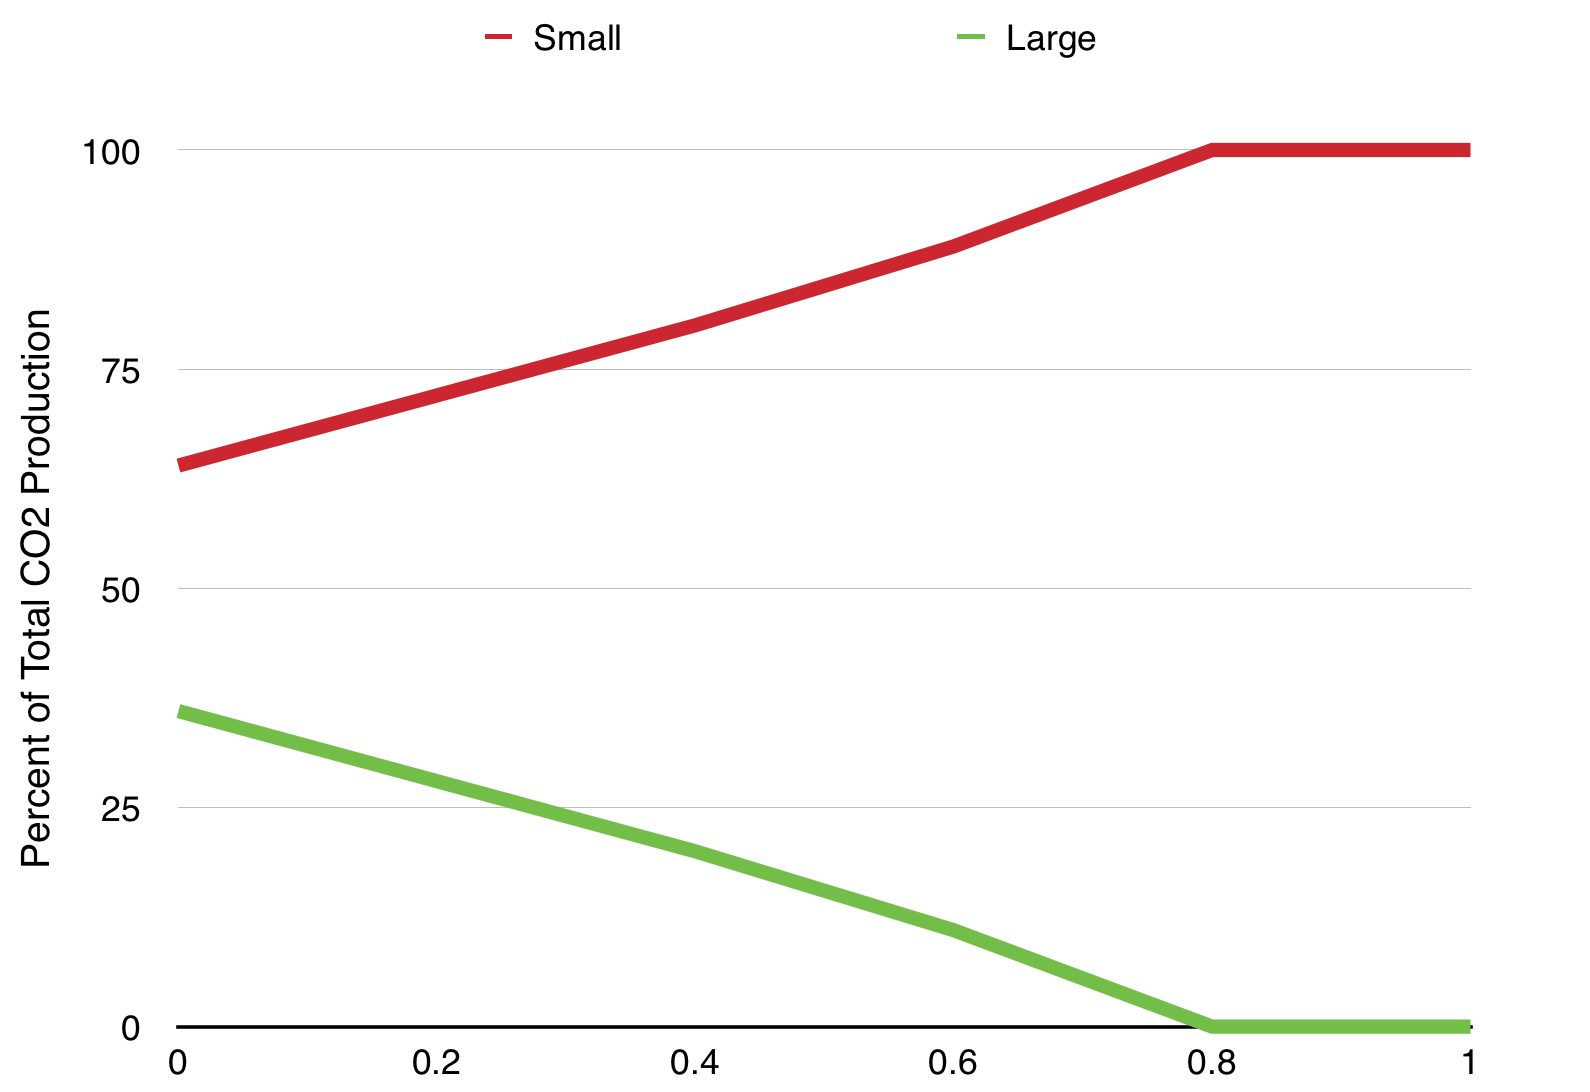
\includegraphics[scale=.4]{CO2_percent.png}
	\caption{Percent of Carbon Produced as Function of Marginal Tax Rate}
	\label{co2percent}
	\end{center}
\end{figure}

The hypothesis was not validated by the model, however. As the carbon tax was ramped up, both small and large producer's production were equally effected. The size of the overall market and the shape of the demand curve were the deciding factors in the production bundles. The large producer could supply the majority of the market using non-emitting technologies, while the smaller counter party couldn't. This lead to the smaller player producing the entirety of the carbon content, while the larger producer was able to make up for the smaller margins by increased volume. 

The results of this experiment suggest that policy actions such as a marginal tax on production will be effective independent of the size of the firms affected. 


\section{Conclusions}
The model can be used effectively to show the benefits of competition in a market (\cref{competetion}), and to a lesser extent, how a carbon effects different players in market (\cref{carbon}). \*

As the number of players increases, the price decreases, thus falling in line with predefined expectations on how competition works in the marketplace. This result not only serves to validate the model and its methodology, but also illustrates the difficulties of high dimensional optimization problems in general. In the case of the model, five\footnote{Which is to say 10, since both the production and the composition are to be predicted for each player} is the maximum number of producers that can lead to a Pareto Optimal outcome. \Cref{numP} shows that at five market participants, the marginal gain in \emph{Total Utility} is negative, going from $77$ to $74$. 


\subsection{Problems with the Model} \label{problems}
While to model can be used to demonstrate the effects of competition in oligopolistic energy markets and the associated changes in carbon production, a number of problems exist. Agents in the model see the output of all competitors as a homogenous sum, and cannot account for individual production. The grouping of output as stated above is a limitation since changes in an individual production cannot be accounted for, i.e. only a single damping function exists, as opposed to a personalized function for all market participants. Multiple damping functions adds increased complexity, but also introduces increased numerical instability. Multiple damping functions could, however, allow for agents to identify the cost and utility structures of the other players, eventually leading to globally optimal solution. Such an algorithm could utilize changes in opponent's production to fit the cost and utility coefficients via multivariate regression. Agent's  would therefore be increasing the accuracy of their predictions at each iteration, thereby making the model a truly "smart" model.\*

As mentioned in \Cref{competetion}, the model breaks down when the number of agents is greater than four. This failure arises from the added market dynamic brought about by adding players \footnote{Recall that each player has three outputs that must be predicted}. As the number of players increases, the number of production decisions in an agent's forecasting increases, causing the algorithm's model of the system to become undefined. This problem is more a limitation of the damping algorithm than any valuable economic insight, although it does serve as a nice example of the real-world difficulty of accurately forecasting any type of outcome in a true market \footnote{See "The Curse of Dimensionality"}. A method to bypass this player limit include adding individual damping functions for each player. Alternatively, agents could be given a set of initial expectations regarding opponent production; the entire game could be re-simulated using a different set of initial conditions, thereby increasing the chances of reaching a convergent solution. 

\subsection{Future Work}
Future iterations of the model will include the suggestions mentioned in \Cref{problems}, specifically the creation of multiple initial predictions. Currently, all agent's use their own cost and utility coefficients to create their initial guess, i.e. "based on my preferences, how much supply should the market have?", and then either  or decrease expectations based of this starting point. If a player is significantly off the actual, they will dramatically alter production and will tend to get trapped around that production value. This implementation not only makes the convergence incredibly sensitive to initial conditions, but also suggests that currently agent's are not to finding the globally optimal solution because their initial expectations are misguided. \*

\subsubsection{Integrating with Geographic Location Model}
Previous research has gone into creating an agent based model for firms' decisions as to where to locate new plants. Combined with the production and scaling capabilities of this model, a model for capturing firms' decisions where to locate and of what new generation capabilities should be to maximize long run profit. 


% ==========================APPENDIX========================== % 
\newpage
\appendix

	\section{WireFrame}

		\begin{figure}[ht!]
			\begin{center}
			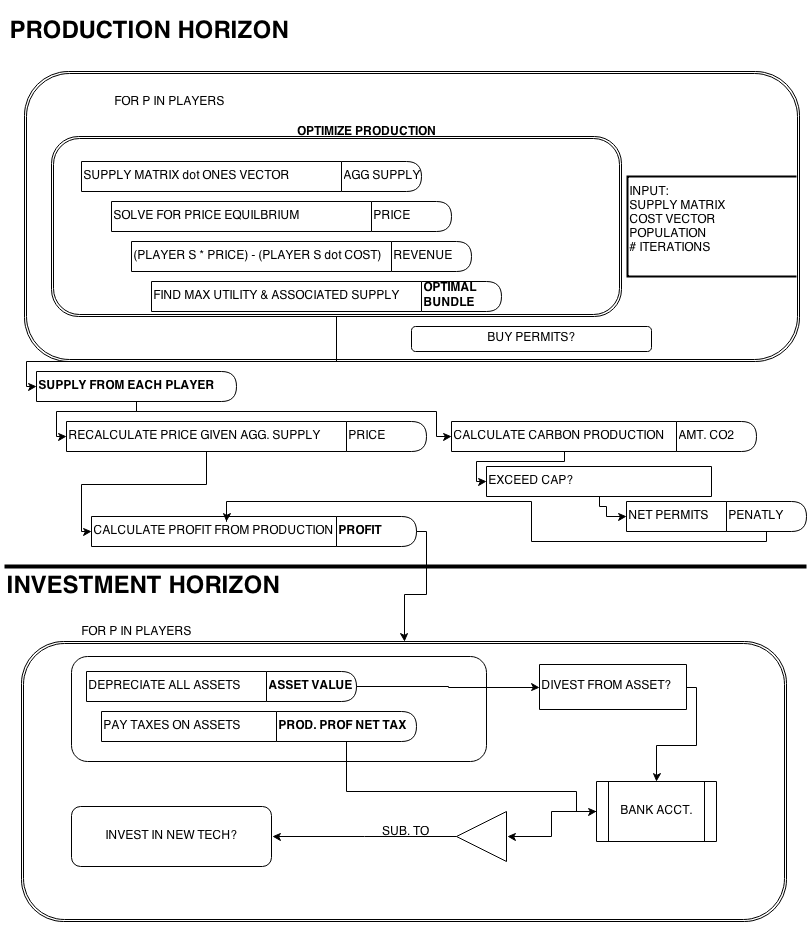
\includegraphics[scale = .5]{wire.png}
			\end{center}
		\end{figure}

\newpage

	\section{Levelized Costs for Power Production}

	\begin{figure}[ht!]
		\begin{center}
		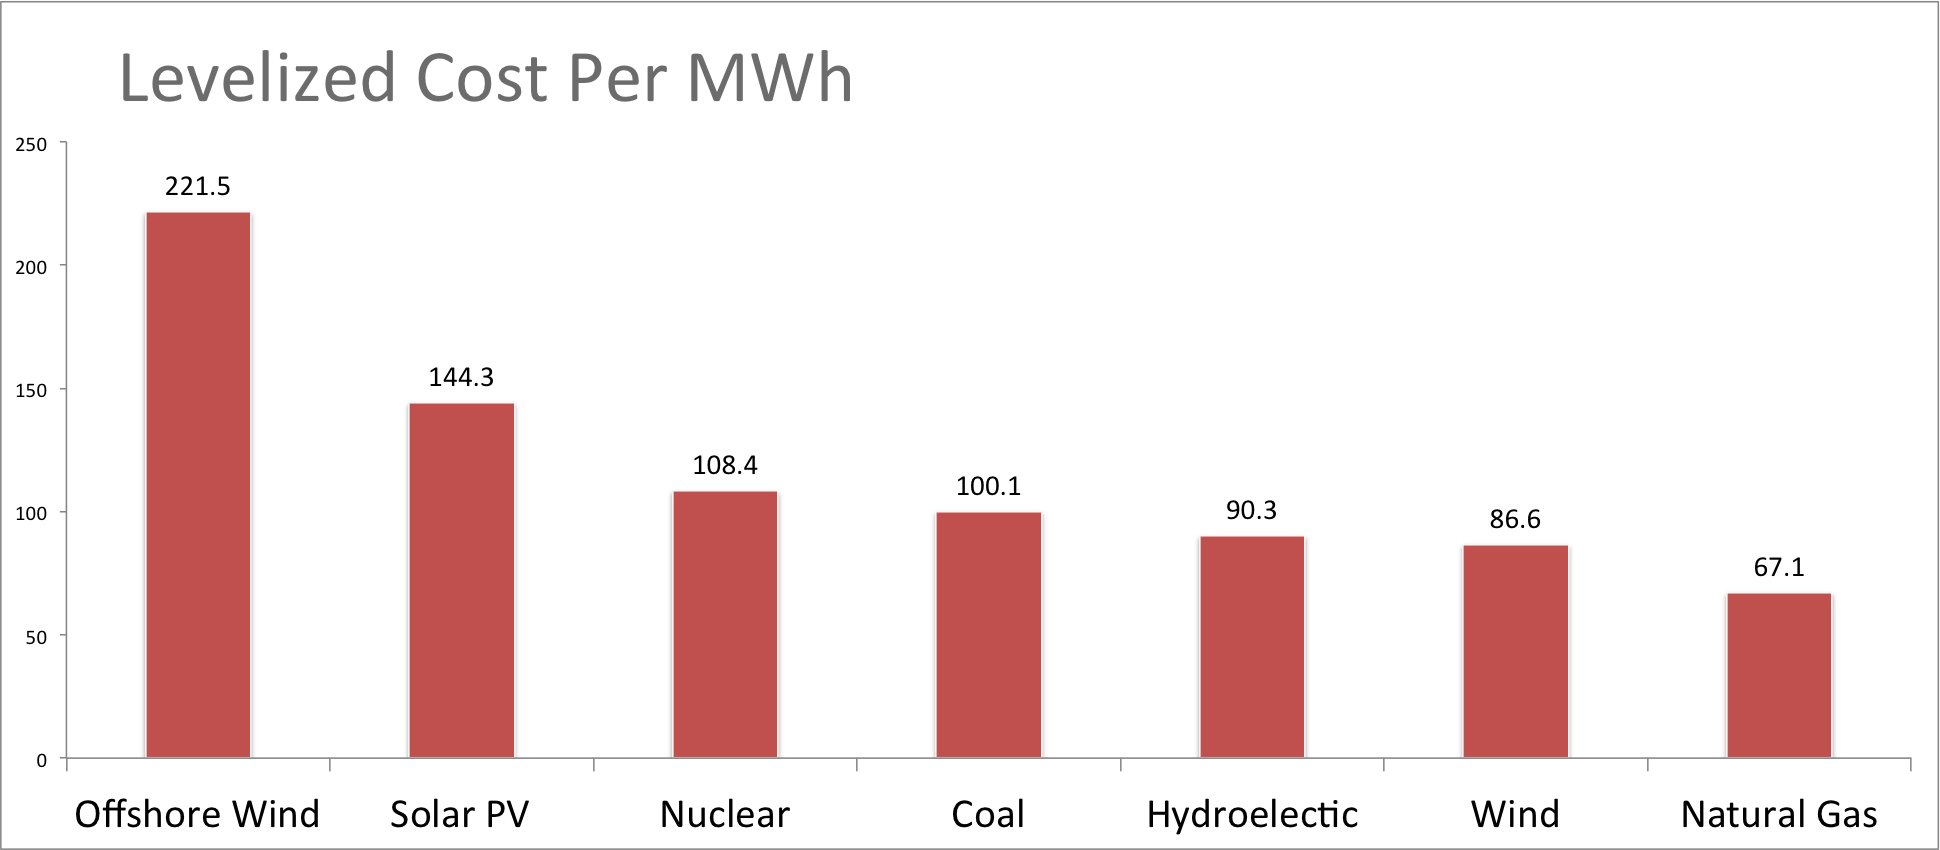
\includegraphics[scale = .5, angle=90]{levelized_cost.png}
		\caption{EPA.gov, 2012 \cite{CO2_Breakdown}}
		\end{center}
		\label{levelized}
	\end{figure}

\newpage


	\section{Two Players}

		\begin{figure}[ht!]
			\begin{center}
			\includegraphics[scale = .6]{2playertotals.eps}
			\end{center}
		\end{figure}


		\begin{figure}[ht!]
			\begin{center}
			\includegraphics[scale = .6]{2player.eps}
			\end{center}
		\end{figure}


\newpage

	\section{Three Players}

		\begin{figure}[ht!]
			\begin{center}
			\includegraphics[scale = .6]{3playertotals.eps}
			\end{center}
		\end{figure}


		\begin{figure}[ht!]
			\begin{center}
			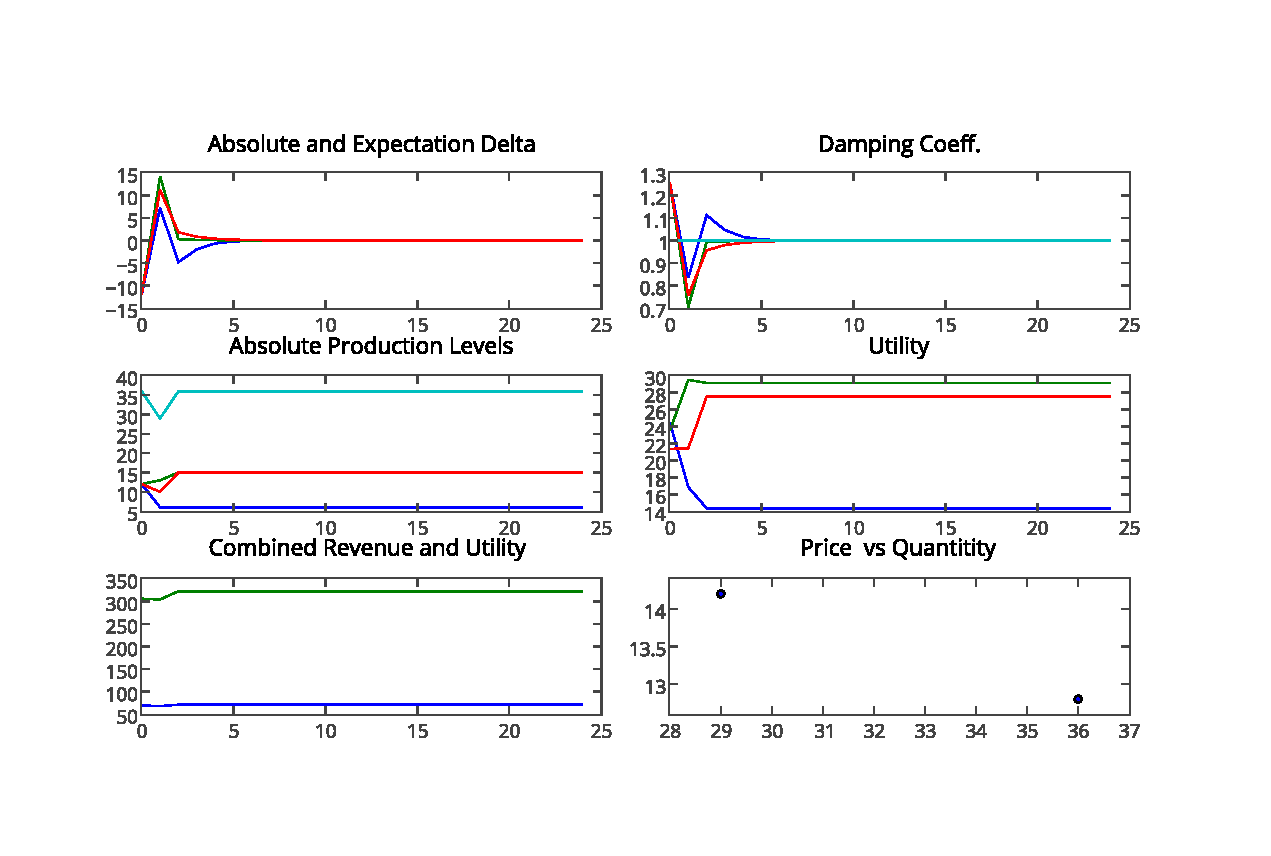
\includegraphics[scale = .6]{3player.eps}
			\end{center}
		\end{figure}


\newpage

	\section{Four Players}

		\begin{figure}[ht!]
			\begin{center}
			\includegraphics[scale = .6]{4playertotals.eps}
			\end{center}
		\end{figure}


		\begin{figure}[ht!]
			\begin{center}
			\includegraphics[scale = .6]{4player.eps}
			\end{center}
		\end{figure}


\newpage

	\section{Five Players} \label{5Players}

		\begin{figure}[ht!]
			\begin{center}
			\includegraphics[scale = .6]{5playertotals.eps}
			\end{center}
		\end{figure}


		\begin{figure}[ht!]
			\begin{center}
			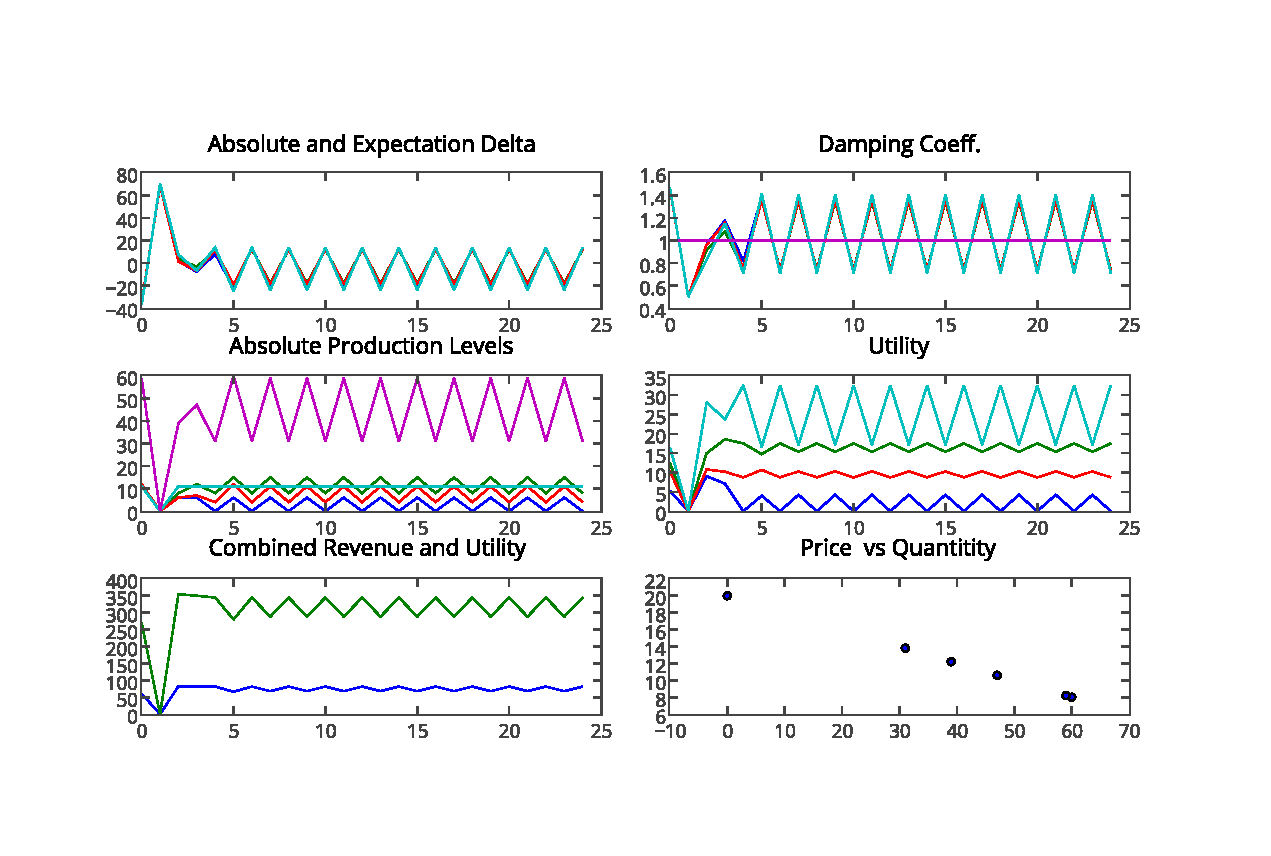
\includegraphics[scale = .6]{5player.eps}
			\end{center}
		\end{figure}


% ==========================BIB========================== % 


\newpage

\begin{thebibliography}{1}

	\bibitem{co2} EIA. ”How Much Carbon Dioxide (CO2) Is Produced hen Different Fuels Are Burned?”” U.S Energy Information Administration. U.S Energy Information Administration, n.d. Web. 9 Dec.2013.

	\bibitem{competetive} Osborne, Martin J. "Competitive Equilibrium in an Exchange Economy." Economics UToronto. U Toronto, 1997. Web. 30 Nov. 2014. \*
	\textless https://www.economics.utoronto.ca/osborne/2x3/tutorial/CEFRM.HTM \textgreater.

	\bibitem{pigou} Sandmo, Agnar (2008). "Pigouvian taxes," \emph{The New Palgrave Dictionary of Economics}, 2nd Edition.

	\bibitem{flowfig} Chappin, Dijkema (2007). "An Agent Based Model of the System of Electricity Production Systems: Exploring the Impact of CO2 Emission-Trading."

	\bibitem{Temps} UCAR. "How Much Has the Global Temperature Risen in the Last 100 Years?" \emph{University Corporation for Atmospheric Research}. UCAR, n.d. Web. 9 Dec. 2013. 


	\bibitem{co2tax} Air quality board to fine Bay Area polluters, San Francisco Chronicle, May 22, 2008.

	\bibitem{games} Sarin, R., and F. Vahid, 2001. "Predicting how People Play Games: A Simple Dynamic Model of Choice." \emph{Games and Economic Behavior}, 34, 104-122.


	\bibitem{hogan} W.W Hogan,"A market power model with strategic interaction in electcity networks," Energy J. vol. 18, no. 5, pp. 107-141, 1997

	\bibitem{chen} H. Chen, P. Wong \emph{et al},"Analyzing oligopolistic electricity market using coevolutionary computation," IEEE Transactions on Power Systems, vol. 21, no. 1, Feb. 2006

	\bibitem{EMCAS} Argonne National Laboratory. "Electricity Market Complex Adaptive System." 
     Argonne National Laboratory. N.p., n.d. Web. 1 Feb. 2015. 
     \textless http://www.dis.anl.gov/projects/emcas.html\textgreater. 

     \bibitem{CO2_Breakdown} EPA. "Overview of Greenhouse Gasses." \emph{EPA}. United States Environmental Protection Agency, n.d. Web. 9 Dec. 2013.


     \bibitem{bunn} Bunn, D.W and F.S Oliveira, 2001. "Agent-based Simulation: An application to the New Electricity Trading Arrangments of England and Wales." \emph{IEEE Transactions on Evoloutionary Computations} 5{5}:493-502

     \bibitem{guerci} Guerci, E., S. Ivaldi, S. Pastore, and S. Cincotti, 2005. "Modeling and Implementation of an Artificial Electricity Market Using Agent-based Technology". \emph{Physica A-Statistical Mechanics and Its Applications}, 355 (1): 69-76.

     \bibitem{pineau}Pineau, P.-O., and P. Murto, 2003. "An Oligopolistic Investment Model of the Finnish Electricity Market." \emph{Annals of Operations Research}, 121, 123-148.
\end{thebibliography}



\end{document} 
